\documentclass[12pt,a4paper]{extarticle}
\usepackage[margin=1in]{geometry}
\usepackage[utf8]{inputenc}
\usepackage{booktabs} % for toprule, midrule and bottomrule
\usepackage{adjustbox}
\usepackage{amsmath}
\usepackage{bbold}
\usepackage{etoolbox}
\usepackage{setspace} % for \onehalfspacing and \singlespacing macros
\usepackage[hidelinks]{hyperref}
\usepackage{array}
\usepackage{graphicx}
\usepackage{setspace}
\usepackage{caption}
\usepackage{pdflscape}
\usepackage{caption}
\usepackage{tabularx}
\usepackage{authblk}
\usepackage{float}
\usepackage{siunitx}
\usepackage{titlesec}
\usepackage{pgfplots}
\usepackage[authoryear]{natbib}
\usepackage{scrextend}
\usepackage{nicefrac}
\usepackage{enumitem}
%\usepackage{showframe}
%\usepackage{lipsum}

% set space
%\doublespacing

% section headings
\renewcommand{\thesection}{\Roman{section}.\hspace{-0.5em}}
\renewcommand\thesubsection{\Alph{subsection}.\hspace{-0.5em}}
\renewcommand\thesubsubsection{\hspace{-1em}}

\titleformat{\section}
{\bf\centering\large}{\thesection}{1em}{}

\titleformat{\subsection}
{\itshape\centering}{\thesubsection}{1em}{}

\titleformat{\subsubsection}
{\bf}{\thesubsubsection}{1em}{}

% unicode chars for plots
\DeclareUnicodeCharacter{2212}{$-$}

% booktabs
\setlength\heavyrulewidth{0.06em} % 0.01em> midrule

% images
\graphicspath{ {D:/Users/saketh/Documents/GitHub/BECCS-Case-Study/documents/exhibits/} }

% array
\newcolumntype{L}[1]{>{\raggedright\let\newline\\\arraybackslash\hspace{0pt}}m{#1}}
\newcolumntype{C}[1]{>{\centering\let\newline\\\arraybackslash\hspace{0pt}}m{#1}}
\newcolumntype{R}[1]{>{\raggedleft\let\newline\\\arraybackslash\hspace{0pt}}m{#1}}

% caption set up
\captionsetup[table]{
	font = {sc},
	labelfont = {bf}
}

% sig stars
\def\sym#1{\ifmmode^{#1}\else\(^{#1}\)\fi}

% hyperlinks
\hypersetup{
	colorlinks=true,
	linkcolor = blue,
	urlcolor  = blue,
	citecolor = blue,
	anchorcolor = blue
}

% bibliography
\makeatletter
\renewenvironment{thebibliography}[1]
{\section*{References}%
	\@mkboth{\MakeUppercase\refname}{\MakeUppercase\refname}%
	\list{}%
	{\setlength{\labelwidth}{0pt}%
		\setlength{\labelsep}{0pt}%
		\setlength{\leftmargin}{\parindent}%
		\setlength{\itemindent}{-\parindent}%
		\@openbib@code
		\usecounter{enumiv}}%
	\sloppy
	\clubpenalty4000
	\@clubpenalty \clubpenalty
	\widowpenalty4000%
	\sfcode`\.\@m}
{\def\@noitemerr
	{\@latex@warning{Empty `thebibliography' environment}}%
	\endlist}
\makeatother

% etoolbox
\AtBeginEnvironment{quote}{\singlespacing}

\begin{document}
	
%	\title{\singlespacing{\textbf{%%%}}}
%	
%	\author[]{Saketh Aleti}
%	
%	\affil[]{\small{%%%}}
%	
%	\date{\vspace{-1em}\small{%%%}}
%	
%	\maketitle
	
	
\section{Literature Outline}

Two classifications for elasticities of substitution

\begin{itemize}
	\item \textbf{Gross/net elasticities}: 
	\begin{itemize}
		\item Net elasticities are computed holding output constant
		\item Gross elasticities are computed by letting output vary optimally (gross)
	\end{itemize}
	\item \textbf{Scalar, asymmetric ratio, or symmetric ratio elasticities}
	\begin{itemize}
		\item Scalar elasticities (Allen-Uzawa) measure the effect of a change in the price of another factor scaled by its cost share on the quantity of a factor demanded
		\item Asymmetric ratio elasticities (Morishima) measure the effect on the factor input ratio of a change in a ratio of prices
		\item Symmetric elasticities can be found by putting restrictions on asymmetric elasticities; holding cost constant on the Morishima elasticities produces the shadow elasticities of substitution
	\end{itemize} 
\end{itemize} 

\subsection{Formulas}

\subsubsection{Translog}

Own price elasticities are given by:
$$\eta_{ii} = \frac{\partial \ln X_i(y, p)}{\partial \ln p_i} = \frac{\beta_{ii} + S_i^2 - S_i}{S_i}
\quad \implies \quad n_{ii}(1, \mathbb{1}) = \frac{\beta_{i,i} - \beta_i^2 - \beta_i}{\beta_i}$$
where $X_i$ is demand for input $i$, $p_i$ is its price, and $S_i$ is its predicted cost share. And, $B_{ij}$ is the second order parameter from the translog cost function, $y$ is the output, and $p$ is a vector of factor prices. 


Cross price elasticities are given by:
$$\eta_{ij} = \frac{\partial \ln X_i(y, p)}{\partial \ln p_j} = \frac{B_{ij} + S_iS_j }{S_i}
\quad \implies \quad n_{ii}(1, \mathbb{1}) = \frac{\beta_{i,i} - \beta_{j}\beta_{i}}{\beta_i}$$
where $B_i$ is the first-order parameter of the translog cost function. 

\subsubsection{Morishima}

The elasticity of substitution here is given by:
$$\mu_{ij} = \left. \frac{\partial \ln(X_j(y, p) / X_i(y,p))}{\partial \ln(p_i/p_j)} \right|_{p_j} = \eta_{ji} - \eta_{ii}$$

\subsubsection{Shadow}

The shadow elasticity of substitution is given by:
$$\sigma_{ij} = \left. \frac{\partial \ln(X_j(y, p) / X_i(y,p))}{\partial \ln(p_i/p_j)} \right|_{C} = \frac{S_i}{S_i + S_j} \mu_{ij} + \frac{S_j}{S_i + S_j} \mu_{ji}$$


\pagebreak

\section{Model of Electricity Production/Consumption}

\subsection{Formulation}

The model involves a consumer and producers reaching equilibrium in a two-period setting. The consumer maximizes a Cobb-Douglas utility function, and the producers allocate capital into two energy sources: one which provides a constant output and the other which generates an intermittent output. 
The producers' energy output, say kWh, at time $t$ is 
$$Y_t = \xi_{1,t} X_1 + \xi_{2,t} X_2$$
where $X_1$ is investment into the constant output source, $X_2$ is the investment into the intermittent output source, and $\xi_{i,t}$ is the conversion factor from input $X_i$ into kWh at time $t$. Referring to the next period as period $s$, we also have:
$$Y_s = \xi_{1,s} X_1 + \xi_{2,s} X_2$$
Since $X_1$ is a constant output source, $\xi_{1,t} = \xi_{1,s}$. And, since $X_2$ is an intermittent source, we may have $\xi_{2,t} > \xi_{2,s}$ without loss of generality. For example, $X_1$ may be coal and $X_2$ may be solar. Letting $\xi_{2,t} > \xi_{2,s}$  reflects the fact that the conversion rate from tons of coal to kWh is independent of the time of day, while the conversion rate for solar panels into kWh is higher during the day. 
Next, the cost of production for inputs $X_i$ is given by:
$$C(X_1, X_2) = p_1 (X_1 - c_1)^{\eta_1} + p_2 (X_2 - c_1)^{\eta_2}$$
where $p_i > 0$, $c_i > 0$, $\eta_i > 2$. When $\eta_i = 3$, this particular function has:
\begin{align*}
\partial C / \partial X_i &> 0 \\
\partial^2 C / \partial X_i^2 &< 0 \text{ when } X_i < c_i \\
\partial^2 C / \partial X_i^2 &> 0 \text{ when } X_i > c_i
\end{align*}
which shows concave costs followed by convex costs. That is, average cost initially decreases with production and then increases. This might be more realistic, but the following results can also be obtained with $c_i = 0$ and $\eta = 2$ which is a simpler model with linearly increasing average costs. 
Lastly, the producer has the following profit function:
$$\Pi = p_t Y_t + p_s Y_2 - C(X_1, X_2)$$
And, the consumer maximizes utility while constrained by their budget:
$$U = Y_t^\alpha \cdot Y_s^\beta$$
$$\text{s.t. }  p_t Y_t + p_s Y_2 \leq B$$




\subsection{Numerical Solution}

First, we assume that the social planner maximizes utility while keeping profit non-negative. Additionally, we keep all prices and quantities non-negative. 


Optimizing a Cobb-Douglas function implies that the demand for energy is given by:
\begin{align*}
Q_{D, t} &= \alpha*B / p_t \\
Q_{D, s} &= \beta*B / p_s
\end{align*}
These demand functions maximize utility while ensuring the consumer budget constraint is satisfied. 

The energy production functions remain the same:
\begin{align*}
Q_{S, t} &= \xi_{1,t} X_1 + \xi_{2,t} X_2 \\
Q_{S, s} &= \xi_{1,s} X_1 + \xi_{2,s} X_2
\end{align*}

But, the producer profit is now:
$$\Pi = p_t \min(Q_{D,t}, Q_{S,t}) + p_s \min(Q_{D,s}, Q_{S,s}) - C(X_1, X_2)$$

Running an optimization routine provides the following results:

\begin{center}
	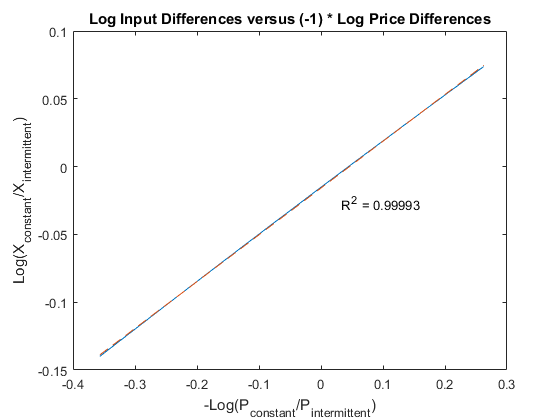
\includegraphics[width=0.9\textwidth]{exhibits/model_v1_ex.png} 
\end{center}

Graphed above is $\ln(X_1/ X_2)$ versus $\ln(P_2/P_1)$. The blue line shows the results while the dashed orange line is an OLS fit. Similar to a CES function, this relationship is practically linear; error may be due to the optimization routine. The results were generated with $p_1 = 10, c_1 = 0.5, c_2 = 0.5, , \eta_1 = 3, \eta_2 = 3, \xi_{1,t} = 5, \xi_{1,s} = 5, \xi_{2,t} = 10, \xi_{2,s}  = 4, \alpha = 0.3, \beta = 0.7, B = 50$, and with $p_2$ allowed to vary over iterations from $7$ to $13$. That is, with:
\begin{align*}
U &= Y_t^{0.3} \cdot Y_s^{0.7} \\
p_t Y_t + p_s Y_2 &\leq 50 \\
Y_t &= 5 X_1 + 10 X_2 \\
Y_s &= 5 X_1 + 4 X_2 \\
C &= 10 (X_1 - 0.5)^{3} + p_2 (X_2 - 0.5)^{3}
\end{align*}

Running the routine again but with $\xi_{1,t} =  \xi_{1,s} = 6$, we get the following results: 

\begin{center}
	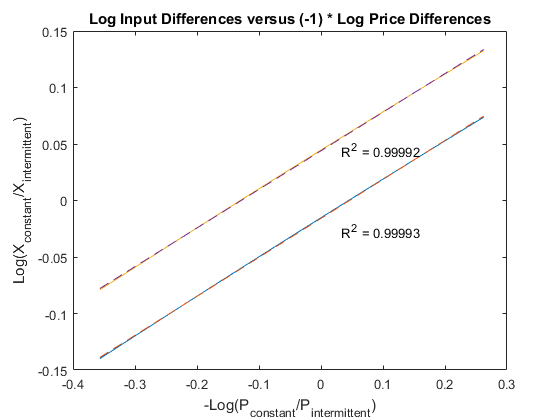
\includegraphics[width=0.9\textwidth]{exhibits/model_v1_ex2.png} 
\end{center}


In the graph above, the yellow line is a second set of results obtained by modifiying $\xi$. We can see that the intercept has shifted without changing the slope very much ($<1\%$ change in the slope), which is similar to what would be seen with a CES model. That is, the optimization of a standard CES model would result in 
$$\ln(X_i/ X_j) = \sigma \ln(P_j / P_i) + \sigma \ln(\xi_i/ \xi_j)$$
where changes in $\xi$ would affect the intercept but not the slope (elasticity of substitution) $\sigma$ as seen in this two-period model. The estimated coefficient of the slope $\hat{\sigma}$ with these parameters is $0.3416$. This implies that the constant and intermittent energy sources are complements in energy production, which reflects reality since an intermittent source could not substitute well for a constant output source. 

Part of the reason the model implies that they are complements may be due to the fact that the cost functions show increasing average cost, so it would be more expensive to completely substitute one for the other. However setting $\eta_1 = \eta_2 = 2$, results in $\hat{\sigma} = 0.6695$. The two are much weaker complements but still remain complements even if average cost is linearly increasing. Generally, as $\eta_i$ decreases, the elasticity of substitution rises and the two become increasingly better substitutes. On the other hand, when the output of the second source becomes more intermittent, when $\xi_{2_d} / \xi_{2_n}$ increases, the elasticity of substitution declines as expected. 

Overall, this result - the near linear relationship between the log of inputs and prices - essentially implies that we could approximate a two-period model of electricity into a one-period model by using a CES production function. This is useful, because we do not have electricity output by source, hour, and state for 2016. Since modeling intermittency directly with a multi-period SAM would be impossible without data to estimate the parameters, a single period SAM with this theoretical approach would be more persuasive. Additionally, using a CES function without $\sigma \to \infty \iff \phi \to 1$ would always imply that 1 kWh from one source does not substitute for 1 kWh from another. When estimating the CES function: 
$$Y = \theta \cdot \left( \Pi_i \alpha_i X_i^\phi \right)^{1/\phi}$$
the estimates will always have $\hat{\theta} \to 1$, $\hat{\alpha_i}$ approaching the average conversion factors, and $\hat{\phi} \to 1$. When the electricity data comes from a single period, such as 2016 in our data, this must be the result; even theoretically this is true. For instance, this is true with the MATLAB simulation when aggregating the two-period model data into one period and fitting a CES function. We see $\theta \to 1$, $\phi \to 1$, and $\alpha_i \to (\xi_{i,t} + \xi_{i,s})/2$.  To get $\hat{\phi} \neq 1$ would be wrong in any single period model, but would make sense in a multi-period model. Implementing this in a CGE would still imply that 1 kWh of solar stops translating into 1 kWh of electricity when a shock occurs. But, this can make sense if we suppose reality follows a multi-period model and such a kWh of solar was just over-generated in one period as a result of optimal investment targeting all periods. So, starting from a multi-period theoretical foundation would better justify using $\phi \neq 1$ in the CGE.

\pagebreak	
%\section*{References}

\subsection{Centralized Approach}

\subsubsection{Cobb-Douglas Utility}

Firstly, the demand function for each commodity is derived from the Cobb-Douglas utility function. Hence, we have:
$$Y_t = (\alpha \cdot B)/p_t \qquad Y_s = (\beta \cdot B)/p_s$$
Therefore, the consumer surplus is given by:
$$\text{CS} = \int_{p_t}^{\infty} (\alpha \cdot B)/p \,dp \; + \; \int_{p_s}^{\infty} (\beta \cdot B)/p \,dp$$
Equivalently, using inverse demand, we have:
$$\text{CS} = \int_{0}^{Y_t} (\alpha \cdot B)/y \,dy \; + \; \int_{0}^{Y_s} (\beta \cdot B)/y \,dy$$
Producer surplus remains equivalent to profit; here I use a simple cost function. 
$$\text{PS} = \Pi = p_t Y_t + p_s Y_2 - ( p_1 X_1^2 + p_2 X_2^2)$$
Then, total welfare is $W = \text{PS} + \text{CS}$. So, we have:
$$\frac{\partial W}{\partial X_1} = \frac{\partial CS}{\partial X_1} + \frac{\partial PS}{\partial X_1} $$
Working with consumer surplus, we get:
\begin{align*}
CS &= (\alpha \cdot B) \cdot (\ln(Y_t) - \ln(0)) + (\beta \cdot B) \cdot (\ln(Y_s) - \ln(0)) \\
&\implies  \frac{\partial CS}{\partial X_1} = (\alpha \cdot B) \cdot (\xi_{1,t} / Y_t) + (\beta \cdot B) \cdot (\xi_{1,s} / Y_s)\\
&\implies  \frac{\partial CS}{\partial X_2} = (\alpha \cdot B) \cdot (\xi_{2,t} / Y_t) + (\beta \cdot B) \cdot (\xi_{2,s} / Y_s)
\end{align*}
And, for profit, we have:
$$ \frac{\partial PS}{\partial X_1} = p_t \cdot \xi_{1,t} + p_s \cdot \xi_{1,s} - 2\, p_1 X_1 $$
$$ \frac{\partial PS}{\partial X_2} = p_t \cdot \xi_{2,t} + p_s \cdot \xi_{2,s} - 2\, p_2 X_2 $$
Hence, the first-order conditions are:
\begin{align*}
\frac{\partial W}{\partial X_1} = 0 &\implies (\alpha \cdot B) \cdot (\xi_{1,t} / Y_t) + (\beta \cdot B) \cdot (\xi_{1,s} / Y_s) + p_t \cdot \xi_{1,t} + p_s \cdot \xi_{1,s} - 2\, p_1 X_1 = 0 \\
\frac{\partial W}{\partial X_2} = 0 &\implies (\alpha \cdot B) \cdot (\xi_{2,t} / Y_t) + (\beta \cdot B) \cdot (\xi_{2,s} / Y_s) + p_t \cdot \xi_{2,t} + p_s \cdot \xi_{2,s} - 2\, p_2 X_2 = 0
\end{align*}


\subsection{Decentralized Solution}

To restate the problem, we have production determined by:
$$Y_t = \xi_{1,t} X_1 + \xi_{2,t} X_2$$
$$Y_s = \xi_{1,s} X_1 + \xi_{2,s} X_2$$
with the cost function $C(X_1, X_2) = p_1 X_1^2 + p_2 X_2^2$. And, the consumer attempts to maximize their utility:
$$U = Y_t^\alpha \cdot Y_s^\beta$$  
subject to $p_t Y_t + p_s Y_s = B$. 



\subsubsection{Cobb-Douglas Utility}

First, assume producers maximize profit. Then, we have:
\begin{align*}
\frac{\partial PS}{\partial X_1} &= p_t \cdot \xi_{1,t} + p_s \cdot \xi_{1,s} - 2\, p_1 X_1 = 0 \\
\frac{\partial PS}{\partial X_2} &= p_t \cdot \xi_{2,t} + p_s \cdot \xi_{2,s} - 2\, p_2 X_2 = 0 \\
\implies X_1 &= \left(p_t \cdot \xi_{1,t} + p_s \cdot \xi_{1,s}\right) / (2 p_1)    \\
\implies X_2 &= \left(p_t \cdot \xi_{2,t} + p_s \cdot \xi_{2,s}\right) / (2 p_2)
\end{align*}
Thus, given the demand curves,
$$Y_t = (\alpha \cdot B)/p_t \qquad Y_s = (\beta \cdot B)/p_s$$
we substitute in $X_1$ and $X_2$ to get:
\begin{align*}
p_t &= \frac{\alpha \cdot B}{\dfrac{\xi_{1,t}(p_s \cdot \xi_{1,s} + p_t \cdot \xi_{1,t})}{2p_1} + \dfrac{\xi_{2,t}(p_s \cdot \xi_{2,s} + p_t \cdot \xi_{2,t})}{2p_2}} \\
p_t &= \frac{\beta \cdot B}{\dfrac{\xi_{1,s}(p_s \cdot \xi_{1,s} + p_t \cdot \xi_{1,t})}{2p_1} + \dfrac{\xi_{2,s}(p_s \cdot \xi_{2,s} + p_t \cdot \xi_{2,t})}{2p_2}}
\end{align*}

Returning to the utility function, $U = Y_t^\alpha \cdot Y_s^\beta$, we expand it to get:
$$U = (\xi_{1,t} X_1 + \xi_{2,t} X_2)^\alpha (\cdot \xi_{1,s} X_1 + \xi_{2,s} X_2)^\beta$$
Furthermore, assuming profit-maximizing firms, we have:
\begin{align*}
U = \; & \left(\xi_{1,t} \left(p_t \cdot \xi_{1,t} + p_s \cdot \xi_{1,s}\right) / (2 p_1) + \xi_{2,t} \left(p_t \cdot \xi_{2,t} + p_s \cdot \xi_{2,s}\right) / (2 p_2) \right)^\alpha \\
&* \left( \xi_{1,s} \left(p_t \cdot \xi_{1,t} + p_s \cdot \xi_{1,s}\right) / (2 p_1) + \xi_{2,s} \left(p_t \cdot \xi_{2,t} + p_s \cdot \xi_{2,s}\right) / (2 p_2) \right)^\beta
\end{align*}


\subsubsection{CES Utility}

Suppose instead that we have a utility function of the form:
$$U = (\alpha Y_t^\phi \, + \, \beta Y_s^\phi)^{1/\phi}$$
The demand functions are then:
\begin{align*}
Y_t &= \left(\frac{\alpha}{p_t}\right)^\sigma \cdot \frac{B}{\alpha^\sigma p_t^{1-\sigma} \, + \, \beta^\sigma p_s^{1-\sigma}} \\
Y_s &= \left(\frac{\beta}{p_s}\right)^\sigma \cdot \frac{B}{\alpha^\sigma p_t^{1-\sigma} \, + \, \beta^\sigma p_s^{1-\sigma}}
\end{align*}
where $\sigma = 1 / (1 - \phi)$ is the elasticity of substitution. And, same as before, we have the following supply curve:
\begin{align*}
X_1^* &= \left( p_t \cdot \xi_{1,t} + p_2 \cdot \xi_{1,s} \right) / (2 p_1) \\
X_2^* &= \left( p_t \cdot \xi_{2,t} + p_2 \cdot \xi_{2,s} \right) / (2 p_2) 
\end{align*}
  
  
\subsubsection{Simpler Model}


	

Suppose that we have the same production function but our first input is equally productive at time $t$ or $s$, so we have:
$$Y_t = \xi_{1} X_1 + \xi_{2,t} X_2$$
$$Y_s = \xi_{1} X_1 + \xi_{2,s} X_2$$
Using matrix notation, we have:
$$M = 
\begin{pmatrix}
\xi_1 & \xi_{2,t} \\
\xi_1 & \xi_{2,s}
\end{pmatrix}
\quad \implies \quad 
Y = M \, X \quad \implies \quad X = M^{-1} \, Y$$

Additionally, suppose that we have the cost function $C = (X_1^2  + X_2^2) / 2$. Then, we have:
\begin{align*}
\frac{\partial C}{\partial Y_t} &= M^{-1}_{11} \cdot X_1 +  M^{-1}_{21} \cdot X_2 \\
\frac{\partial C}{\partial Y_s} &= M^{-1}_{12} \cdot X_1 +  M^{-1}_{22} \cdot X_2 
\end{align*}
Then, with our original profit function, we get the following first order conditions
\begin{align*}
\Pi &= p_t Y_t + p_s Y_s - C(X_1, X_2) \\
\implies p_t &= M^{-1}_{11} \cdot X_1 +  M^{-1}_{21} \cdot X_2 \\
\implies p_y &= M^{-1}_{12} \cdot X_1 +  M^{-1}_{22} \cdot X_2 \\
\implies P &= (M^{-1})^{T} X \\
\implies X &= M^{T} P
\end{align*}
Therefore, our supply curve is $Y = M \, M^{T} P$. 
And, assuming Cobb-Douglas utility, we have:
$$Y_t = (\alpha \cdot B)/p_t \qquad Y_s = (\beta \cdot B)/p_s $$
Hence, setting supply equal to demand, we get:
\begin{align*}
M \, M^{T} P &= 
\begin{pmatrix}
\alpha \cdot B / p_t \\
\beta \cdot B / p_s
\end{pmatrix} \\
\iff 
\left(\begin{array}{cc} {\xi _{1}}^2+{\xi _{2,t}}^2 & {\xi _{1}}^2+\xi _{2,s}\,\xi _{2,t}\\ {\xi _{1}}^2+\xi _{2,s}\,\xi _{2,t} & {\xi _{1}}^2+{\xi _{2,s}}^2 \end{array}\right) 
\begin{pmatrix}
p_t \\
p_s
\end{pmatrix}  
&= \begin{pmatrix}
\alpha \cdot B / p_t \\
\beta \cdot B / p_s
\end{pmatrix} \\
\implies
Y_{supply} &= 
\begin{pmatrix}
(\xi _{1}^2+\xi _{2,t}^2)p_t +  (\xi _{1}^2+\xi _{2,s}\,\xi _{2,t})p_s \\[2ex]
(\xi _{1}^2+\xi _{2,s}\,\xi _{2,t}) p_t  + ({\xi _{1}}^2+\xi _{2,s}^2 ) p_s
\end{pmatrix}\\
\implies
Y_{demand} &= 
\begin{pmatrix}
\alpha \cdot B / p_t \\
\beta \cdot B / p_s
\end{pmatrix} 
\end{align*}
Expanding and simplifying, we have:
\begin{align*}
({\xi _{1}}^2+\xi _{2,t}^2)p_t^2 +  (\xi _{1}^2+\xi _{2,s}\,\xi _{2,t})p_s p_t &= \alpha \cdot B \\
({\xi _{1}}^2+\xi _{2,s}\,\xi _{2,t}) p_t p_s + ({\xi _{1}}^2+\xi _{2,s}^2 ) p_s^2 &= \beta \cdot B \\
\implies ({\xi _{1}}^2+\xi _{2,t}^2)p_t^2 - ({\xi _{1}}^2+\xi _{2,s}^2 ) p_s^2 &= (\alpha - \beta) \cdot B
\end{align*}
Similarly, solving for the supply and demand of $X$, we get:
\begin{align*}
X_{demand} = 
\begin{pmatrix}
\dfrac{\mathrm{B}\,\left(\alpha \,p_{s}\,\xi _{2,s}-\beta\,p_{t}\,\xi _{2,t}\right)}{p_{s}\,p_{t}\,\xi _{1}\,\left(\xi _{2,s}-\xi _{2,t}\right)}\\[3ex] -\dfrac{\mathrm{B}\,\left(\alpha \,p_{s}-\beta\,p_{t}\right)}{p_{s}\,p_{t}\,\left(\xi _{2,s}-\xi _{2,t}\right)}
\end{pmatrix}  \qquad
X_{supply} = 
\begin{pmatrix}
p_{s}\,\xi _{1}+p_{t}\,\xi _{1}\\[1ex]
 p_{s}\,\xi _{2,s}+p_{t}\,\xi _{2,t}
\end{pmatrix}
\end{align*}
	

\subsubsection{Simplest Model}
	
	
Suppose that we have the same production function but our first input is equally productive at time $t$ or $s$, so we have:
$$Y_t = \xi_{1} X_1 + \xi_{2,t} X_2$$
$$Y_s = \xi_{1} X_1 + \xi_{2,s} X_2$$
Using matrix notation, we have:
$$M = 
\begin{pmatrix}
\xi_1 & \xi_{2,t} \\
\xi_1 & \xi_{2,s}
\end{pmatrix}
\quad \implies \quad 
Y = M \, X \quad \implies \quad X = M^{-1} \, Y$$
Additionally, suppose we have linear cost: $C = p_1 X_1 + p_2 X_2$. 
Then, our first-order conditions for profit maximization, assuming linear cost, are:
\begin{align*}
\frac{\partial PS}{\partial X_1} &= p_t \cdot \xi_1  + p_s \cdot \xi_1 - p_1 = 0 \\
\frac{\partial PS}{\partial X_2} &= p_t \cdot \xi_{2,t}  + p_s \cdot \xi_{2,s} - p_2 = 0 \\
\implies M^T p &= 
\begin{pmatrix}
p_1 \\
p_2
\end{pmatrix} \\
\implies p &= (M^{T})^{-1} \begin{pmatrix}
p_1 \\
p_2
\end{pmatrix}
\end{align*}
This essentially means that we have a supply curve that is perfectly horizontal at the optimal prices. Consequently, profit must be zero. 
$$
p^{opt} = 
\begin{pmatrix}
p_t^{opt} \\
p_s^{opt}
\end{pmatrix}
=
\begin{pmatrix}
\dfrac{p_{2}\,\xi _{1}-p_{1}\,\xi _{2,s}}{\xi _{1}\,\left(\xi _{2,t}-\xi _{2,s}\right)}\\[2ex]
-\dfrac{p_{2}\,\xi _{1}-p_{1}\,\xi _{2,t}}{\xi _{1}\,\left(\xi _{2,t}-\xi _{2,s}\right)}
\end{pmatrix}
$$
Then, assuming utility maximization, we have the following first-order conditions:
\begin{align*}
Y_t &= (\alpha \cdot B) / (p_t) \\
Y_s &= (\beta \cdot B) / (p_s)
\end{align*}
Therefore, the optimal quantities of $Y$ are given by:
\begin{align*}
Y^{opt} = 
\begin{pmatrix}
Y_t^{opt} \\
Y_s^{opt} 
\end{pmatrix}
=
\begin{pmatrix}
-\dfrac{\alpha \,\mathrm{B}\,\xi _{1}\,\left(\xi _{2,s}-\xi _{2,t}\right)}{p_{2}\,\xi _{1}-p_{1}\,\xi _{2,s}}\\[2.5ex]
\dfrac{\beta\,\mathrm{B}\,\xi _{1}\,\left(\xi _{2,s}-\xi _{2,t}\right)}{p_{2}\,\xi _{1}-p_{1}\,\xi _{2,t}}
\end{pmatrix}
\end{align*}
Lastly, since $Y = MX$,the optimal quantities of $X$ are given by:
\begin{align*}
X^{opt} = 
\begin{pmatrix}
X_1^{opt} \\
X_1^{opt} 
\end{pmatrix}
=
M^{-1} \, Y^{opt} = 
\begin{pmatrix}
-\dfrac{\mathrm{B}\,\left(\alpha \,p_{2}\,\xi _{1}\,\xi _{2,s}-\alpha \,p_{1}\,\xi _{2,s}\,\xi _{2,t}+\beta\,p_{2}\,\xi _{1}\,\xi _{2,t}-\beta\,p_{1}\,\xi _{2,s}\,\xi _{2,t}\right)}{\left(p_{2}\,\xi _{1}-p_{1}\,\xi _{2,s}\right)\,\left(p_{2}\,\xi _{1}-p_{1}\,\xi _{2,t}\right)}\\[3ex] 
\dfrac{\alpha \,\mathrm{B}\,\xi _{1}}{p_{2}\,\xi _{1}-p_{1}\,\xi _{2,s}}+\dfrac{\beta\,\mathrm{B}\,\xi _{1}}{p_{2}\,\xi _{1}-p_{1}\,\xi _{2,t}}
\end{pmatrix}
\end{align*}
Now, to find the comparative statics, we return to the first order conditions:
\begin{alignat*}{2}
&\frac{\partial PS}{\partial X_1} &&= p_t \cdot \xi_1  + p_s \cdot \xi_1 - p_1 = 0 \\
&\frac{\partial PS}{\partial X_2} &&= p_t \cdot \xi_{2,t}  + p_s \cdot \xi_{2,s} - p_2 = 0 \\ 
&\implies 
&&\begin{pmatrix}
\xi_1 & \xi_1 \\
\xi_{2,t} & \xi_{2,s} 
\end{pmatrix}
\begin{pmatrix}
p_t \\
p_s
\end{pmatrix}
=
\begin{pmatrix}
p_1 \\
p_2
\end{pmatrix} \\
&\implies 
&&
\begin{pmatrix}
p_t \\
p_s
\end{pmatrix}
=
\begin{pmatrix} 
\frac{\xi _{2,s}}{\xi _{1}\,\xi _{2,s}-\xi _{1}\,\xi _{2,t}} & -\frac{1}{\xi _{2,s}-\xi _{2,t}}\\ 
-\frac{\xi _{2,t}}{\xi _{1}\,\xi _{2,s}-\xi _{1}\,\xi _{2,t}} & \frac{1}{\xi _{2,s}-\xi _{2,t}} 
\end{pmatrix}
\begin{pmatrix}
p_1 \\
p_2
\end{pmatrix}
\end{alignat*}

Letting $N$ be the last matrix which provides the solutions to $p_t$ and $p_s$, we have the following derivatives and short-hand notations:
\begin{alignat*}{2}
\frac{\partial N}{\partial \xi_1} &= 
\left(\begin{array}{cc} \frac{\xi _{2,s}}{{\xi _{1}}^2\,\left(\xi _{2,t}-\xi _{2,s}\right)} & 0\\ -\frac{\xi _{2,t}}{{\xi _{1}}^2\,\left(\xi _{2,t}-\xi _{2,s}\right)} & 0 \end{array}\right)
&&\equiv N^{\xi_1} \\
\frac{\partial N}{\partial \xi_{2,t}} &=
\left(\begin{array}{cc} \frac{\xi _{2,s}}{\xi _{1}\,{\left(\xi _{2,s}-\xi _{2,t}\right)}^2} & -\frac{1}{{\left(\xi _{2,s}-\xi _{2,t}\right)}^2}\\ -\frac{\xi _{2,s}}{\xi _{1}\,{\left(\xi _{2,s}-\xi _{2,t}\right)}^2} & \frac{1}{{\left(\xi _{2,s}-\xi _{2,t}\right)}^2} \end{array}\right)
&&\equiv N^{\xi_{2,t}} \\
\frac{\partial N}{\partial \xi_{2,s}} &=
\left(\begin{array}{cc} -\frac{\xi _{2,t}}{\xi _{1}\,{\left(\xi _{2,s}-\xi _{2,t}\right)}^2} & \frac{1}{{\left(\xi _{2,s}-\xi _{2,t}\right)}^2}\\ \frac{\xi _{2,t}}{\xi _{1}\,{\left(\xi _{2,s}-\xi _{2,t}\right)}^2} & -\frac{1}{{\left(\xi _{2,s}-\xi _{2,t}\right)}^2} \end{array}\right)
&&\equiv N^{\xi_{2,s}} 
\end{alignat*}

By utility maximization, we have:
\begin{align*}
Y_t = (\alpha \cdot B)/p_t \qquad Y_s = (\beta \cdot B)/p_s 
\end{align*}
Therefore, we have:
\begin{align*}
\frac{\partial Y_t}{\partial \xi_1} = \frac{\partial Y_t}{\partial p_t}  \cdot \frac{\partial p_t}{\partial \xi_1} = (-(\alpha \cdot B)/p_t^2) \cdot (N^{\xi_1}_{1,1} p_1 + 0 \, p_2) < 0 \\
\frac{\partial Y_s}{\partial \xi_1} = \frac{\partial Y_s}{\partial p_s}  \cdot \frac{\partial p_s}{\partial \xi_1} = (-(\beta \cdot B)/p_s^2) \cdot (N^{\xi_1}_{2,1} p_1 + 0 \, p_2) > 0 
\end{align*}
because $N^{\xi_1}_{2,1} < 0 < N^{\xi_1}_{1,1}$ since we assumed earlier that $\xi_{2,t} > \xi_{2,s}$. If we have $X_1$ being coal and $X_2$ being solar, we have improvements in the conversion rate of coal to energy causing shifts in energy production to the night (period $s$) and away from the day (period $t$). 


Now, we can do the same for $\xi_{2,t}$. 
\begin{align*}
\frac{\partial Y_t}{\partial \xi_{2,t}} = \frac{\partial Y_t}{\partial p_t}  \cdot \frac{\partial p_t}{\partial \xi_{2,t}} = (-(\alpha \cdot B)/p_t^2) \cdot (N^{\xi_{2,t}}_{1,1} p_1 + N^{\xi_{2,t}}_{1,2} \cdot p_2) \\
\frac{\partial Y_s}{\partial \xi_{2,t}} = \frac{\partial Y_s}{\partial p_s}  \cdot \frac{\partial p_s}{\partial \xi_{2,t}} = (-(\beta \cdot B)/p_s^2) \cdot (N^{\xi_{2,t}}_{2,1} p_1 + N^{\xi_{2,t}}_{2,2} \cdot p_2) 
\end{align*}
Firstly, note that $N^{\xi_{2,t}}_{1,1} \, p_1 + N^{\xi_{2,t}}_{1,2} \, p_2 < 0$ when $\xi_1 / p_1 > \xi_{2,s} / p_2$. And note that the second row of $N^{\xi_{2,t}}$ is simply the negative of the first row; hence, $N^{\xi_{2,t}}_{1,1} \, p_1 + N^{\xi_{2,t}}_{1,2} \, p_2 > 0$ when $\xi_1 / p_1 > \xi_{2,s} / p_2$. In practice, $\xi$ represents the conversion rate from units of input to units of output and $p$ is the price. So, the condition $\xi_1 / p_1 > \xi_{2,s} / p_2$ simply states that the cost efficiency of input $1$ is greater than the cost efficiency of input $2$ during period $s$. Therefore, we have:
$$\xi_1 / p_1 > \xi_{2,s} / p_2 \implies 
\frac{\partial Y_s}{\partial \xi_{2,t}} < 0 < \frac{\partial Y_t}{\partial \xi_{2,t}} $$
If $X_1$ were coal and $X_2$ were solar, we would obviously have coal being more cost efficient at night than solar. Therefore, improvements to solar's efficiency during the day would shift energy production to the day and away from the night. 

Lastly, we have the derivatives for $\xi_{2,s}$. 
\begin{align*}
\frac{\partial Y_t}{\partial \xi_{2,s}} = \frac{\partial Y_t}{\partial p_t}  \cdot \frac{\partial p_t}{\partial \xi_{2,s}} = (-(\alpha \cdot B)/p_t^2) \cdot (N^{\xi_{2,s}}_{1,1} p_1 + N^{\xi_{2,s}}_{1,2} \cdot p_2) \\
\frac{\partial Y_s}{\partial \xi_{2,s}} = \frac{\partial Y_s}{\partial p_s}  \cdot \frac{\partial p_s}{\partial \xi_{2,s}} = (-(\beta \cdot B)/p_s^2) \cdot (N^{\xi_{2,s}}_{2,1} p_1 + N^{\xi_{2,s}}_{2,2} \cdot p_2) 
\end{align*}
Here, recall that we have  $\xi_{2,s} \, N^{\xi_{2,s}} = - \xi_{2,t} \, N^{\xi_{2,t}}$, which helps carry through the previous algebra. That is, replacing $\xi_{2,s}$ with $\xi_{2,t}$ and flipping the signs, we get:
$$\xi_1 / p_1 < \xi_{2,t} / p_2 \implies 
\frac{\partial Y_s}{\partial \xi_{2,s}} < 0 < \frac{\partial Y_t}{\partial \xi_{2,s}} $$
So, if solar is more cost efficient during the day than coal, then improvements in the night-time efficiency of solar will increase energy output during the day and decrease it during the night. This is because solar becoming more efficient will result in greater solar usage and so energy production will reflect the lop-sided output of solar. 

It's important to note that the change in $Y_t$ and $Y_s$ in response to other parameters always gives away whether we consume more or less of $X_2$. This is because $X_1$ has a fixed conversion rate, so $Y_t$ and $Y_s$ will move in the same direction if $X_1$ changes. But, they can only move in opposite directions if $X_2$ changes. For example, if we have $\xi_{2,t} > \xi_{2,s}$, then an increase in $Y_t$ and a decrease in $Y_s$ must signal a greater use of $X_2$ and less of $X_1$. 


Next, we have the comparative statics for the inputs $X_1$ and $X_2$. By definition, we have:
\begin{alignat*}{1}
Y &= MX \\
\implies X &= M^{-1} \, Y \\
&= \begin{pmatrix}
\dfrac{\xi _{2,t}\,Y_{s}-\xi _{2,s}\,Y_{t}}{\xi _{1}\,\left(\xi _{2,t}-\xi _{2,s}\right)}\\[2ex] 
\dfrac{Y_{t}-Y_{s}}{\xi _{2,t}-\xi _{2,s}} 
\end{pmatrix}
\end{alignat*}
Now, we differentiate with respect to the $\xi$ parameters. Using the previous derivations for the derivatives of $Y$ assumes utility and profit maximization.
\begin{alignat*}{2}
&\frac{\partial X_1}{\partial \xi_1} &&= - X_1 / \xi_1 + \left(\xi_{2,t} \, \frac{\partial Y_s}{\partial \xi_{1}} - \xi_{2,s} \, \frac{\partial Y_t}{\partial \xi_{1}} \right) \cdot \left(\xi_1 \, (\xi_{2,t} - \xi_{2,s}))^{-1} \right)  \\
&\frac{\partial X_1}{\partial \xi_{2,t}} &&= -X_1/(\xi_1 \, (\xi_{2,t} - \xi_{2,s})) + \left( - \xi_{2,s} \, \frac{\partial Y_t}{\partial \xi_{2,t}} + \xi_{2,t} \, \frac{\partial Y_s}{\partial \xi_{2,t}} + Y_s \right)\cdot(\xi_1 \, (\xi_{2,t} - \xi_{2,s}))^{-1} \\
&\frac{\partial X_1}{\partial \xi_{2,s}} &&= X_1/(\xi_1 \, (\xi_{2,t} - \xi_{2,s})) + \left( - \xi_{2,s} \, \frac{\partial Y_t}{\partial \xi_{2,s}} + \xi_{2,t} \, \frac{\partial Y_s}{\partial \xi_{2,s}} - Y_t \right)\cdot(\xi_1 \, (\xi_{2,t} - \xi_{2,s}))^{-1}  \\
\end{alignat*}
The above inequalities assume $Y_t \geq Y_s$, which must always be true given $\xi_{2,t} > \xi_{2,s}$, and the last inequality assumes $\xi_1 / p_1 < \xi_{2,t} / p_2$. The first inequality is negative since we proved earlier that $\frac{\partial Y_t}{\partial \xi_1} < 0 < \frac{\partial Y_s}{\partial \xi_1}$. Similarly, we get the result for the last inequality using the results for the derivatives of $Y_t$ and $Y_s$. The second inequality may be positive or negative. 
Next, for $X_2$, we have:
\begin{alignat*}{2}
&\frac{\partial X_2}{\partial \xi_1} &&= 
\left( \frac{\partial Y_t}{\partial \xi_{1}} -  \frac{\partial Y_s}{\partial \xi_{1}} \right) \cdot (\xi_{2,t} - \xi_{2,s}) < 0 \\
C_2 \implies &\frac{\partial X_1}{\partial \xi_{2,t}} &&= \left(\frac{\partial Y_t}{\partial \xi_{2,t}} - \frac{\partial Y_s}{\partial \xi_{2,t}}\right)/(\xi_{2,t} - \xi_{2,s}) - (Y_t - Y_s)/(\xi_{2,t} - \xi_{2,s})^2 > 0 \\
&\frac{\partial X_2}{\partial \xi_{2,s}} &&= \left(\frac{\partial Y_t}{\partial \xi_{2,s}} - \frac{\partial Y_s}{\partial \xi_{2,s}}\right)/(\xi_{2,t} + \xi_{2,s}) - (Y_t - Y_s)/(\xi_{2,t} - \xi_{2,s})^2 
\end{alignat*}
$$\text{where} \quad C_2 \iff \left(\frac{\partial (Y_t - Y_s)}{\partial \xi_{2,t}} \cdot \frac{\xi_{2,t} - \xi_{2,s}}{(Y_t - Y_s)} > 1\right) \; \wedge \; \left(\xi_1 / p_1 > \xi_{2,s} / p_2 \right)$$
Note that $C_2$ may or may not be true. 

\subsection{Example Two Period Case with CD Utility and Two Technologies}

Suppose our utility function is instead given by $Y_t^{\alpha_t} \, Y_s^{\alpha_s}$ where our two periods are $t$ and $s$. Optimizing utility given the budget constraint $Y_t p_t + Y_s p_s = I$, our demand curves are $Y_t = \alpha_t / p_t$ and $Y_s = \alpha_s / p_s$. 

Next, we introduce the following matrices to simplify the notation: 
$$
Y = \begin{pmatrix}
Y_t \\
Y_s 
\end{pmatrix}
\quad 
P = \begin{pmatrix}
p_t \\
p_s 
\end{pmatrix}
\quad 
X = \begin{pmatrix}
X_1 \\
X_2 
\end{pmatrix}
\quad 
\xi = \begin{pmatrix}
\xi _{\mathrm{1t}} & \xi _{\mathrm{2t}}\\ \xi _{\mathrm{1s}} & \xi _{\mathrm{2s}}
\end{pmatrix}$$
where $X_i$ is the quantity of input technologies and $\xi_{it}$ is the output of technology $i$ at time $t$. This implies that our output $Y = \xi \,X$. Next, we have profit maximizing firms with linear cost. Suppose $c_i$ is the cost of each unit of technology $i$, and let $C$ be a vector of $c_i$. Then, our profit function is:
$$\Pi = P^T \, Y - C^T \, X = \left(P^T \, \xi - C^T   \right)\, X$$
Now, assuming that $\xi$ is invertible, we have the first order condition:
\begin{align*}
P^T\, \xi &= C^T \\
P &= (\xi^{-1})^T \, C  \\
P^{opt} &= \begin{pmatrix}
-\dfrac{c_{1}\,\xi _{\mathrm{2s}}-c_{2}\,\xi _{\mathrm{1s}}}{\xi _{\mathrm{1s}}\,\xi _{\mathrm{2t}}-\xi _{\mathrm{1t}}\,\xi _{\mathrm{2s}}}  \\[2ex]
\dfrac{c_{1}\,\xi _{\mathrm{2t}}-c_{2}\,\xi _{\mathrm{1t}}}{\xi _{\mathrm{1s}}\,\xi _{\mathrm{2t}}-\xi _{\mathrm{1t}}\,\xi _{\mathrm{2s}}} 
\end{pmatrix}
\end{align*}
Substituting back into the FOC for consumer demand, we have:
$$
Y^{opt} = \begin{pmatrix}
\dfrac{\alpha _{t}\,\left(\xi _{\mathrm{1s}}\,\xi _{\mathrm{2t}}-\xi _{\mathrm{1t}}\,\xi _{\mathrm{2s}}\right)}{c_{2}\,\xi _{\mathrm{1s}} - c_{1}\,\xi _{\mathrm{2s}}} \\[2ex]
\dfrac{\alpha _{s}\,\left(\xi _{\mathrm{1s}}\,\xi _{\mathrm{2t}}-\xi _{\mathrm{1t}}\,\xi _{\mathrm{2s}}\right)}{c_{1}\,\xi _{\mathrm{2t}}-c_{2}\,\xi _{\mathrm{1t}}} 
\end{pmatrix}
\implies 
X^{opt} = \begin{pmatrix}
\dfrac{\alpha _{t}\,\xi _{\mathrm{2s}}}{c_{1}\,\xi _{\mathrm{2s}}-c_{2}\,\xi _{\mathrm{1s}}}+\dfrac{\alpha _{s}\,\xi _{\mathrm{2t}}}{c_{1}\,\xi _{\mathrm{2t}}-c_{2}\,\xi _{\mathrm{1t}}} \\[2ex] 
-\dfrac{\alpha _{t}\,\xi _{\mathrm{1s}}}{c_{1}\,\xi _{\mathrm{2s}}-c_{2}\,\xi _{\mathrm{1s}}}-\dfrac{\alpha _{s}\,\xi _{\mathrm{1t}}}{c_{1}\,\xi _{\mathrm{2t}}-c_{2}\,\xi _{\mathrm{1t}}}
\end{pmatrix}
$$
If we assume that $Y$ is positive in both periods, then, without loss of generality, we have:
\begin{align*}
\text{$X_1$ has a comparative advantage in producing in period $s$: } \quad 
{\xi_{1s}}/{\xi_{1t}} &> {\xi_{2s}}/{\xi_{2t}} \\
\text{$X_1$ is more cost effective at producing in period $s$: } \quad \xi_{1s}/c_1 &> \xi_{2s}/c_2  \\
\text{$X_2$ is more cost effective at producing in period $t$:} \quad \xi_{1t}/c_t &< \xi_{2t}/c_2
\end{align*}
Similarly, if we assume $X$ is positive for both technologies, then, without loss of generality, we have:
\begin{align*}
\alpha_t \xi_{2s} \left( c_1 \xi_{2t} - c_2 \xi_{1t} \right) &> \alpha_s \xi_{2t} \left( c_2 \xi_1s - c_1 \xi_2s \right) \\
\alpha_t \xi_{1s} \left( c_1 \xi_{2t} - c_2 \xi_{1t} \right) &< \alpha_s \xi_{1t} \left( c_2 \xi_1s - c_1 \xi_2s \right) \\
\implies \xi_{2s} / \xi_{1s} &> \xi_{2t}/ \xi_{1t}
\end{align*}


\subsection{Two Period Two Technology Case with Risk}

The intermittency of electricity technologies not only concerns when they produce but how consistently they can produce. 
Consider the same simplified, two-period model as before with technologies that produce according to a stochastic process. Specifically, suppose that $X_1$ produces at the rate $N(\xi_{1t}, \sigma_{1t}^2)$ in period $t$ and at the rate $N(\xi_{1s}, \sigma_{1s}^2)$ in period $s$; also, consider equivalent definitions for $X_2$. We use the following matrices to simplify notation:
$$
\xi = 
\begin{pmatrix}
\xi _{\mathrm{1t}} & \xi _{\mathrm{2t}}\\ \xi _{\mathrm{1s}} & \xi _{\mathrm{2s}}
\end{pmatrix}
\quad 
\Sigma_t = \begin{pmatrix}
\sigma_{1t}^2 & \sigma_{1t, 2t} \\ 
\sigma_{1t, 2t} & \sigma_{2t}^2
\end{pmatrix}
\quad 
\Sigma_s = \begin{pmatrix}
\sigma_{1s}^2 & \sigma_{1s, 2s} \\ 
\sigma_{1s, 2s} & \sigma_{2s}^2
\end{pmatrix}
\quad 
$$
where $\Sigma_t$ is the covariance of electricity production in period $t$ and likewise for $\Sigma_s$ at period $s$; we the generation processes in both periods are independent for simplicity. This essentially reduces to a portfolio maximization problem in each period; however, there is a significant difference: electricity demand varies by period and the production technologies' output and variance of output vary by period as well. The optimization problem can be defined as:
\begin{align*}
\max \quad E \left[ U \right] \\
\text{s.t. \quad} I \cdot  w_i / c_i &= X_i \,\, \forall i \\
\textbf{1}^T w_i &= 1 \\
w_i &\in [0,1] \,\, \forall i
\end{align*}
where $w_i$ is the percent of our budget that is spent on $X_1$ and $X_2$, $I$ is the budget, and $c_i$ is the price of $X_i$.  Since the technologies generate electricity according to a normal process, we have:
\begin{equation*}
\mu \equiv
\begin{pmatrix}
\mu_t \\
\mu_s
\end{pmatrix}
=
\xi \, \textbf{w}
\qquad
\sigma_t^2 
=
\textbf{w}^T \,  \Sigma_t \, \textbf{w} \\
\qquad
\sigma_s^2
=
\textbf{w}^T \,  \Sigma_s \, \textbf{w}
\end{equation*}
\vspace{-2em}
\begin{align*}
Y_t &\sim  N \left( \mu_t, \sigma_t^2 \right) \\
Y_s &\sim  N \left( \mu_s, \sigma_s^2 \right)
\end{align*}
where $\textbf{w}$ is a column vector of weights, $\mu$ represents the electricity generation rate in each period, and $\Sigma$ is the covariance matrix for this rate. 
To solve, we take the second-order Taylor series around $(\overline{Y}_t, \overline{Y}_s) \equiv E \left[ Y_t, Y_s \right]$ which represents our average electricity generation. This is given by:
\begin{align*}
U(Y_t, Y_s) &\approx \overline{U} + \overline{U}_t(Y_t - \overline{Y_t}) + \overline{U}_s(Y_s - \overline{Y_s}) \\
&\phantom{\approx} \, + (1/2) \left[ \overline{U}_{tt}(Y_t - \overline{Y_t})^2 + 2 \overline{U}_{ts}(Y_t - \overline{Y_t})(Y_s - \overline{Y_s})  + \overline{U}_{ss}(Y_s - \overline{Y_s})^2 \right]
\end{align*}
where $\overline{U} \equiv U(\overline{Y}_t, \overline{Y}_s)$, and $\overline{U}_t$ is the derivative of $U$ with respect to $Y_t$ evaluated at $\overline{Y}_t$. Taking the expectation, the $U_t$ and $U_s$ drop out since $E(Y_s - \overline{Y_s}) = 0$, and the $U_{ts}$ drops out since $Y_t$ and $Y_s$ are independent so $E\left[(Y_t - \overline{Y_t})(Y_s - \overline{Y_s})\right] = 0 $. Thus, we are left with:
\begin{align*}
E \left[ U(Y_t, Y_s) \right] &\approx \overline{U} + (1/2) \left[\overline{U}_{tt}\,\sigma_t^2 + \overline{U}_{ss}\, \sigma_s^2 \right]
\end{align*}

%In practice, suppose we have $X_1$ as coal and $X_2$ as solar, and lienar costs. Then, we will see the following effects:
%
%\begin{enumerate}[topsep=0pt,itemsep=-1ex,partopsep=1ex,parsep=1ex]
%	\item Improvements in the conversion rate of coal to electricity
%	\begin{enumerate}[topsep=-1ex,itemsep=-1ex,partopsep=1ex,parsep=1ex]
%		\item Decreases the use of solar
%		\item 
%	\end{enumerate}
%	\item Improvements in the conversion rate of solar to electricity during time $t$
%	\begin{enumerate}[topsep=-1ex,itemsep=-1ex,partopsep=1ex,parsep=1ex]
%		\item %
%		\item %
%	\end{enumerate}
%	\item Improvements in the conversion rate of solar to electricity during time $s$
%	\begin{enumerate}[topsep=-1ex,itemsep=-1ex,partopsep=1ex,parsep=1ex]
%		\item %
%		\item %
%	\end{enumerate}
%\end{enumerate} 

	

\pagebreak

\pagebreak
	
	\begin{thebibliography}{9}
		
%		\bibitem[Angel, Harris, and Spatt(2011)]{Angel} 
%		Angel, J.J., Harris, L.E., \& Spatt, C. S. (2011). Equity Trading in the 21st Century. Quarterly Journal Of Finance, 1(1), 1-53.
		
		\bibitem[Stern(2012)]{Stern} 
		Stern, D. (2012). “Interfuel Substitution: A Meta-Analysis.” Journal of Economic Surveys 26 (2): 307–331. \href{https://doi.org/10.1111/j.1467-6419.2010.00646.x}{https://doi.org/10.1111/j.1467-6419.2010.00646.x}.
		
	\end{thebibliography}	
	
\end{document}





